% Options for packages loaded elsewhere
\PassOptionsToPackage{unicode}{hyperref}
\PassOptionsToPackage{hyphens}{url}
\PassOptionsToPackage{dvipsnames,svgnames,x11names}{xcolor}
%
\documentclass[
  number]{elsarticle}

\usepackage{amsmath,amssymb}
\usepackage{iftex}
\ifPDFTeX
  \usepackage[T1]{fontenc}
  \usepackage[utf8]{inputenc}
  \usepackage{textcomp} % provide euro and other symbols
\else % if luatex or xetex
  \usepackage{unicode-math}
  \defaultfontfeatures{Scale=MatchLowercase}
  \defaultfontfeatures[\rmfamily]{Ligatures=TeX,Scale=1}
\fi
\usepackage{lmodern}
\ifPDFTeX\else  
    % xetex/luatex font selection
\fi
% Use upquote if available, for straight quotes in verbatim environments
\IfFileExists{upquote.sty}{\usepackage{upquote}}{}
\IfFileExists{microtype.sty}{% use microtype if available
  \usepackage[]{microtype}
  \UseMicrotypeSet[protrusion]{basicmath} % disable protrusion for tt fonts
}{}
\makeatletter
\@ifundefined{KOMAClassName}{% if non-KOMA class
  \IfFileExists{parskip.sty}{%
    \usepackage{parskip}
  }{% else
    \setlength{\parindent}{0pt}
    \setlength{\parskip}{6pt plus 2pt minus 1pt}}
}{% if KOMA class
  \KOMAoptions{parskip=half}}
\makeatother
\usepackage{xcolor}
\setlength{\emergencystretch}{3em} % prevent overfull lines
\setcounter{secnumdepth}{5}
% Make \paragraph and \subparagraph free-standing
\makeatletter
\ifx\paragraph\undefined\else
  \let\oldparagraph\paragraph
  \renewcommand{\paragraph}{
    \@ifstar
      \xxxParagraphStar
      \xxxParagraphNoStar
  }
  \newcommand{\xxxParagraphStar}[1]{\oldparagraph*{#1}\mbox{}}
  \newcommand{\xxxParagraphNoStar}[1]{\oldparagraph{#1}\mbox{}}
\fi
\ifx\subparagraph\undefined\else
  \let\oldsubparagraph\subparagraph
  \renewcommand{\subparagraph}{
    \@ifstar
      \xxxSubParagraphStar
      \xxxSubParagraphNoStar
  }
  \newcommand{\xxxSubParagraphStar}[1]{\oldsubparagraph*{#1}\mbox{}}
  \newcommand{\xxxSubParagraphNoStar}[1]{\oldsubparagraph{#1}\mbox{}}
\fi
\makeatother


\providecommand{\tightlist}{%
  \setlength{\itemsep}{0pt}\setlength{\parskip}{0pt}}\usepackage{longtable,booktabs,array}
\usepackage{calc} % for calculating minipage widths
% Correct order of tables after \paragraph or \subparagraph
\usepackage{etoolbox}
\makeatletter
\patchcmd\longtable{\par}{\if@noskipsec\mbox{}\fi\par}{}{}
\makeatother
% Allow footnotes in longtable head/foot
\IfFileExists{footnotehyper.sty}{\usepackage{footnotehyper}}{\usepackage{footnote}}
\makesavenoteenv{longtable}
\usepackage{graphicx}
\makeatletter
\def\maxwidth{\ifdim\Gin@nat@width>\linewidth\linewidth\else\Gin@nat@width\fi}
\def\maxheight{\ifdim\Gin@nat@height>\textheight\textheight\else\Gin@nat@height\fi}
\makeatother
% Scale images if necessary, so that they will not overflow the page
% margins by default, and it is still possible to overwrite the defaults
% using explicit options in \includegraphics[width, height, ...]{}
\setkeys{Gin}{width=\maxwidth,height=\maxheight,keepaspectratio}
% Set default figure placement to htbp
\makeatletter
\def\fps@figure{htbp}
\makeatother

\usepackage{booktabs}
\usepackage{caption}
\usepackage{longtable}
\usepackage{colortbl}
\usepackage{array}
\makeatletter
\@ifpackageloaded{float}{}{\usepackage{float}}
\floatstyle{plain}
\@ifundefined{c@chapter}{\newfloat{suppfig}{h}{losuppfig}}{\newfloat{suppfig}{h}{losuppfig}[chapter]}
\floatname{suppfig}{Figure S}
\newcommand*\quartosuppfigref[1]{Figure \hyperref[#1]{S\ref{#1}}}
\@ifpackageloaded{caption}{}{\usepackage{caption}}
\DeclareCaptionLabelFormat{quartosuppfigreflabelformat}{#1#2}
\captionsetup[suppfig]{labelformat=quartosuppfigreflabelformat}
\newcommand*\listofsuppfigs{\listof{suppfig}{List of Supplementary Figures}}
\makeatother
\makeatletter
\@ifpackageloaded{caption}{}{\usepackage{caption}}
\AtBeginDocument{%
\ifdefined\contentsname
  \renewcommand*\contentsname{Table of contents}
\else
  \newcommand\contentsname{Table of contents}
\fi
\ifdefined\listfigurename
  \renewcommand*\listfigurename{List of Figures}
\else
  \newcommand\listfigurename{List of Figures}
\fi
\ifdefined\listtablename
  \renewcommand*\listtablename{List of Tables}
\else
  \newcommand\listtablename{List of Tables}
\fi
\ifdefined\figurename
  \renewcommand*\figurename{Figure}
\else
  \newcommand\figurename{Figure}
\fi
\ifdefined\tablename
  \renewcommand*\tablename{Table}
\else
  \newcommand\tablename{Table}
\fi
}
\@ifpackageloaded{float}{}{\usepackage{float}}
\floatstyle{ruled}
\@ifundefined{c@chapter}{\newfloat{codelisting}{h}{lop}}{\newfloat{codelisting}{h}{lop}[chapter]}
\floatname{codelisting}{Listing}
\newcommand*\listoflistings{\listof{codelisting}{List of Listings}}
\makeatother
\makeatletter
\makeatother
\makeatletter
\@ifpackageloaded{caption}{}{\usepackage{caption}}
\@ifpackageloaded{subcaption}{}{\usepackage{subcaption}}
\makeatother

\ifLuaTeX
  \usepackage{selnolig}  % disable illegal ligatures
\fi
\usepackage[]{natbib}
\bibliographystyle{elsarticle-num}
\usepackage{bookmark}

\IfFileExists{xurl.sty}{\usepackage{xurl}}{} % add URL line breaks if available
\urlstyle{same} % disable monospaced font for URLs
\hypersetup{
  pdftitle={Investigating the Spatial Variability in Soil Geochemical and Colour Properties Across Two Contrasting Land Uses},
  pdfauthor={Maria Luna; Alexander J Koiter; Taras E Lychuk; Arnie Waddel; Alan Moulin},
  pdfkeywords={Soil geochemistry, Soil colour, Spatial analysis},
  colorlinks=true,
  linkcolor={blue},
  filecolor={Maroon},
  citecolor={Blue},
  urlcolor={Blue},
  pdfcreator={LaTeX via pandoc}}


\setlength{\parindent}{6pt}
\begin{document}

\begin{frontmatter}
\title{Investigating the Spatial Variability in Soil Geochemical and
Colour Properties Across Two Contrasting Land Uses}
\author[1]{Maria Luna%
%
}
 \ead{LUNAMIMA56@brandonu.ca} 
\author[2]{Alexander J Koiter%
\corref{cor1}%
}
 \ead{koitera@brandonu.ca} 
\author[3]{Taras E Lychuk%
%
}
 \ead{taras.lychuk@AGR.GC.CA} 
\author[3]{Arnie Waddel%
%
}
 \ead{arnie.waddell@AGR.GC.CA} 
\author[3]{Alan Moulin%
%
}
 \ead{apmaafc7788@gmail.com} 

\affiliation[1]{organization={Brandon University, Masters in
Environmental and Life Sciences},addressline={270 18th
St},city={Brandon},postcode={R7A 6A9},postcodesep={}}
\affiliation[2]{organization={Brandon University, Department of
Geography and Environment},addressline={270 18th
St},city={Brandon},postcode={R7A 6A9},postcodesep={}}
\affiliation[3]{organization={Agriculture and Agri-Food Canada, Brandon
Research and Development Centre},addressline={2701 Grand Valley
Road},city={Brandon},postcode={R7A 5Y3},postcodesep={}}

\cortext[cor1]{Corresponding author}





        
\begin{abstract}
Quantification and accurate assessment of the spatial variability and
distribution of soil physical and biogeochemical properties are vital
components of agri-environmental research and modeling, including
sediment source fingerprinting. Understanding the distribution of soil
properties is crucial in the development of appropriate, reliable, and
efficient sampling campaigns. This study was aimed to investigate the
spatial variability in soil geochemical and colour (i.e., spectral
reflectance) soil properties (\textless63um) across two contrasting land
uses. The main objectives of this study are to: 1) quantify the spatial
variability of geochemical and colour properties at a field-scale
(\textasciitilde{} 40 ha) across agricultural and forested sites; 2)
evaluate the spatial variability and distribution of soil properties and
its relation to seven terrain attributes (e.g., catchment area,
elevation). A combination of univariate analysis and geostatistical
methods were applied to characterize the soil geochemistry and colour
properties. This information was used to both quantify and assess the
variability in soil properties. The variability and spatial
autocorrelation were generally both site and soil property specific. For
a selection of soil properties exhibiting some spatial autocorrelation,
random forest regression was used to indentify the relative importance
of terrain attributes on observed patterns of soil geochemical and
colour properties. Elevation was found to explain the greatest amount of
the variation in soil properties followed by the SAGA wetness index and
relative slope position. These types of information can be used to help
create efficient soil sampling designs by providing information that can
inform sampling locations and number of samples collected in order to
meet research needs and objectives.
\end{abstract}





\begin{keyword}
    Soil geochemistry \sep Soil colour \sep 
    Spatial analysis
\end{keyword}
\end{frontmatter}
    

\section{Introduction}\label{introduction}

Variation in soil biological, chemical, and physical properties occurs
across the landscape and in response to both regional and local (i.e.,
field-scale) variations in parent material, relief or topography,
organisms, climate, time and land use/management (Mulla and McBratney,
2002). Understanding the patterns and drivers for this variation is an
important component of many agri-environmental studies. For example, the
spatial variability in soil properties is a key component for plant
nutrient management plans as investigating the spatial variation
influences how suitable producers sample their fields for fertilization
and compliance with management practices and environmental regulations
(Kariuki et al., 2009).

The spatial variability in soil properties is often caused by changes in
topography that affect the storage and transport of water within the
soil profile (Mulla and McBratney, 2002). The soil variability at a
field-scale might be described by methods of geostatistics and soil
mapping. Geostatistics is a technology used to estimate the soil
property values in non-sampled areas or areas with sparse samplings and
provides a set of statistical tools for a description of spatial
patterns, quantitative modeling of spatial continuity, spatial
prediction, and uncertainty assessment (Goovaerts, 1999). Geostatistical
techniques that incorporate spatial information into predictions can
improve estimation and enhance map quality (Zhang et al., 2007). Most
applications of this statistical technique were estimated in small-scale
areas or on a field-scale with minimal work completed in large land
areas or soil regions even though standard geostatistical techniques
have been suitable for describing the spatial distribution of soil and
to successfully analyze spatial variability of soil properties (Zhang et
al., 2007). Geostatistics is focused on spatial correlation, spatial
interpolation, simulation, and visualization of values of random
variables. Spatial interpolation is commonly used to predict a value of
a variable of interest at unmeasured locations with the available
measurements at sampled sites (Robertson, 2008). Kriging, for instance,
is a multistep method of spatial interpolation, which assumes that the
direction or distance between sample points reflects a spatial
autocorrelation that can be used to explain variation in the surface
(Oliver and Webster, 1990).

The use of semivariograms illustrate the spatial autocorrelation of the
measured sample points at each field. To better understand
semivariograms, three main characteristics are commonly used to describe
these models. The range is the distance where the model first flattens.
For instance, sample locations separated by distances closer than the
range are spatially autocorrelated, whereas locations farther apart than
the range are not. The sill is the value that the semivariogram model
attains at the range (i.e., the value on the y-axis). The nugget refers
to when at zero separation distance, the semivariogram value is zero.
However, at a small separation distance, the semivariogram often
exhibits a nugget effect, which is a value greater than zero (Oliver and
Webster, 1990; Robertson, 2008). Spatial dependency or autocorrelation
is often evaluated in terms of ratio of the nugget to sill expressed in
percentage or proportion. For instance, a low ratio (less than 25\%)
means that a large part of the variance is introduced spatially,
indicating a strong spatial dependency of the variable. A high ratio
(more than 75\%) generally indicates weak spatial dependency; otherwise,
the spatial dependency is considered moderate (25\% - 75\%) (Cambardella
et al., 1994).

From a sediment fingerprinting perspective, investigating the spatial
variability of soil properties at a field-scale can be advantageous to
identify, classify, and distinguish between potential sources of
sediment (Boudreault et al., 2019). However, only some studies have
explored fingerprint variability at individual sampling locations (e.g.,
Du and Walling, 2017; Pulley et al., 2017) as well as over larger scales
(e.g., Wilkinson et al., 2015). Therefore, investigating spatial
variability is not common in fingerprinting studies. The field-scale
variability in fingerprint properties at different scales has been
employed in sediment fingerprinting studies. For example, in a study
conducted by Collins et al.~(2019), determined that the main finding
derives from reported observations on the variability of fingerprint
properties (δ13C, δ15N, and total carbon and nitrogen) that were used at
a field-scale. Observations of variability from the study are related to
sites that present different climates, slopes, soils, and management
characteristics. Because in this study the soil was relatively aerobic
during the sampling period, it is determined that diffusion of gaseous
products (e.g., N and O) thorough the soil profile might be the cause of
having lack of variation in geochemistry between soil layers. Similarly,
in order to estimate the variability of soils fingerprint properties,
topsoil characteristics, such as texture, and organic matter (OM)
content are important data to take into account (Miranda et al., 2006).

The degree of spatial variability in fingerprint properties can be
described by the coefficient of variation (CV) and R2, which is
associated with the semivariogram. A study conducted by Du and Walling
(2017) used radionuclides and geochemistry as the main fingerprint
properties in samples of surface soils that were collected. Results
present a range CV between 10-30\%. Due to the fact that 137Cs fallout
to the study field occurred over a period of 25 years, it was reasonable
to assume that the spatial variation of the 137Cs activity of the
surface soil was reflected by systematic variation related with the
effect of soil redistribution during the sampling period. In the case of
the other fingerprint properties, the variability could be principally
associated with soil redistribution and topography. This study suggests
that erosional history and topography are important aspects of designing
an appropriate sampling approach.

A different study by Zhang et al.~(2007) determined spatial variability
of nutrient properties in black soil of Northeast China. The spatial
variability of organic matter content, total N, and total P was
principally associated with climate and terrain and perhaps the most
possible reason was cultivation and the difference in potassium
fertilizer application. The difference in annual average temperature in
black soil study area was reported to be more than 7°C, which indicated
that temperature could be a significant factor that might influence soil
nutrient mineralization and accumulation. Therefore, at larger spatial
scales, land management history and climate variables are likely
important aspects to consider when investigating variability and
characterizing sources of sediment.

Methods of geostatistics have been developed to estimate spatial
variability of fingerprint and soil physical properties (Goovaerts,
1999). The major application of geostatistics to soil physical
properties include the variability of soil colour, texture, structure,
density, and porosity. Another application of geostatistics includes the
estimation and mapping of soil attributes in unsampled areas. Moreover,
a significant contribution of geostatistics is the assessment of the
uncertainty about unsampled values, which normally takes the form of a
map of the probability of exceeding critical values, such as regulatory
thresholds in soil pollution or soil quality.

Geostatistical analyses allow to quantify the spatial distribution and
variability based on spatial field-scale of the site(s) and spatial
pattern of modeling semivariograms. These models have been broadly
applied to assess spatial correlation in soil properties, including
physical and geochemical properties. The main objectives in this study
are to: 1) quantify the spatial variability in soil geochemical and
colour fingerprint properties at a field-scale across two contrasting
land uses (agriculture and forest) using geostatistics and terrain
analysis; and 2) identify patterns and sources of variability in
fingerprint properties over a large spatial scale. The range of spatial
scales/sampling designs presented are intended to capture variation in
fingerprint properties as part of sediment source fingerprinting
studies.

\section{Methods}\label{methods}

\subsection{Site description}\label{site-description}

\begin{figure}[H]

\centering{

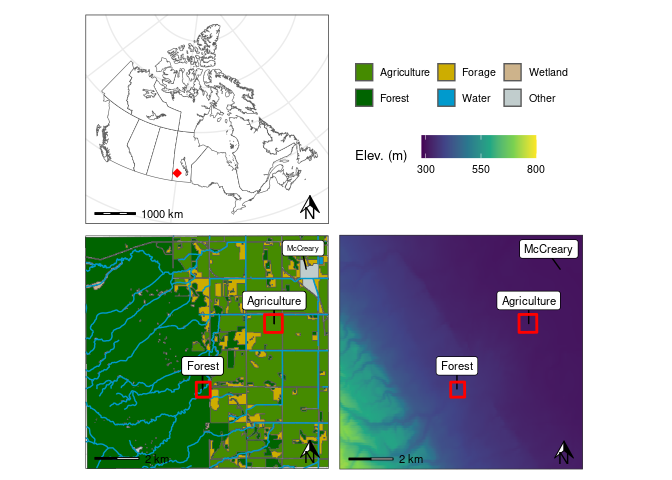
\includegraphics{index_files/figure-latex/notebooks-location_map-fig-location_map-output-2.png}

}

\caption{\label{fig-location_map}Map showing the location of the study
sites within Canada, and the regional land use and topography.}

\end{figure}%

\textsubscript{Source:
\href{https://alex-koiter.github.io/spatial-variability-soil-manuscript/notebooks/location_map.qmd.html\#cell-fig-location_map}{Research
Site Locations}}

\section{Results}\label{results}

\subsection{Univariate summary}\label{univariate-summary}

\begin{longtable}[]{@{}ccccccc@{}}

\caption{\label{tbl-univariate-summary}Summary univariate statistics of
selected geochemical and colour soil properties for each site (n = 49).}

\tabularnewline

\toprule\noalign{}
Property & Mean & SD & Max & Min & Skewness & CV \\
\midrule\noalign{}
\endhead
\bottomrule\noalign{}
\endlastfoot
\multicolumn{7}{@{}c@{}}{%
Agriculture} \\
Ca & 4.00 & 2.19 & 8.78 & 0.95 & 0.28 & 54.66 \\
Co & 8.76 & 0.83 & 10.60 & 7.50 & 0.52 & 9.48 \\
Cs & 0.75 & 0.15 & 1.07 & 0.47 & 0.18 & 19.93 \\
Fe & 1.92 & 0.09 & 2.11 & 1.71 & −0.25 & 4.70 \\
Li & 15.62 & 1.42 & 19.80 & 12.80 & 0.62 & 9.11 \\
La & 18.23 & 1.22 & 20.20 & 15.50 & −0.29 & 6.71 \\
Nb & 0.59 & 0.06 & 0.73 & 0.46 & 0.45 & 9.67 \\
Ni & 29.63 & 2.72 & 35.70 & 25.00 & 0.36 & 9.17 \\
Rb & 18.43 & 4.33 & 26.70 & 10.20 & 0.24 & 23.48 \\
Sr & 91.31 & 38.98 & 163.50 & 38.60 & 0.09 & 42.69 \\
a* & 3.38 & 0.32 & 4.15 & 2.59 & −0.03 & 9.53 \\
b* & 8.84 & 0.97 & 10.59 & 6.69 & −0.18 & 11.00 \\
c* & 9.47 & 1.02 & 11.32 & 7.17 & −0.19 & 10.74 \\
h* & 1.20 & 0.01 & 1.23 & 1.18 & 0.19 & 1.12 \\
x & 0.47 & 0.00 & 0.48 & 0.47 & 0.06 & 0.46 \\
\multicolumn{7}{@{}c@{}}{%
Forest} \\
Ca & 1.89 & 1.53 & 5.46 & 0.47 & 1.07 & 81.12 \\
Co & 6.76 & 1.39 & 9.60 & 4.00 & 0.03 & 20.62 \\
Cs & 0.55 & 0.12 & 0.78 & 0.34 & 0.25 & 21.73 \\
Fe & 1.18 & 0.13 & 1.46 & 0.83 & −0.58 & 11.24 \\
Li & 6.47 & 0.90 & 8.60 & 4.30 & −0.02 & 13.89 \\
La & 15.00 & 2.60 & 21.80 & 10.30 & 0.33 & 17.31 \\
Nb & 0.37 & 0.06 & 0.56 & 0.17 & −0.68 & 17.10 \\
Ni & 18.09 & 3.90 & 28.00 & 11.00 & 0.33 & 21.55 \\
Rb & 13.83 & 1.85 & 18.10 & 9.90 & 0.27 & 13.40 \\
Sr & 32.43 & 12.60 & 64.20 & 15.30 & 0.98 & 38.87 \\
a* & 5.73 & 0.41 & 6.56 & 4.41 & −0.38 & 7.10 \\
b* & 12.47 & 2.01 & 15.91 & 8.02 & 0.22 & 16.11 \\
c* & 13.74 & 1.94 & 17.00 & 9.15 & 0.15 & 14.15 \\
h* & 1.13 & 0.05 & 1.23 & 1.06 & 0.34 & 4.13 \\
x & 0.49 & 0.00 & 0.49 & 0.48 & −0.21 & 0.47 \\

\end{longtable}

\textsubscript{Source:
\href{https://alex-koiter.github.io/spatial-variability-soil-manuscript/notebooks/univariate_summary.qmd.html\#cell-tbl-univariate-summary}{Univariate
summary}}

\begin{longtable}[]{@{}ccccccc@{}}

\caption{\label{tbl-univariate2-summary}Summary statistics for the
interpoloated values (10m resolution) for slected geochemical and colour
soil properties and terrain attributes for each site.}

\tabularnewline

\toprule\noalign{}
Property & Mean & SD & Max & Min & Skewness & CV \\
\midrule\noalign{}
\endhead
\bottomrule\noalign{}
\endlastfoot
\multicolumn{7}{@{}c@{}}{%
Agriculture} \\
Ca & 4.12 & 2.10 & 8.76 & 0.918 & 0.0727 & 51.0 \\
Co & 8.75 & 0.664 & 10.6 & 7.52 & 0.431 & 7.59 \\
Cs & 0.729 & 0.123 & 1.07 & 0.458 & 0.376 & 16.9 \\
Fe & 1.92 & 0.0644 & 2.10 & 1.73 & −0.450 & 3.36 \\
Li & 15.7 & 1.16 & 19.3 & 13.2 & 0.551 & 7.38 \\
La & 18.2 & 0.817 & 19.8 & 16.5 & −0.268 & 4.49 \\
Nb & 0.593 & 0.0550 & 0.740 & 0.459 & 0.569 & 9.27 \\
Ni & 29.9 & 2.23 & 34.5 & 26.3 & −0.0100 & 7.46 \\
Rb & 18.0 & 3.94 & 26.1 & 11.5 & 0.498 & 21.8 \\
Sr & 93.4 & 38.6 & 167 & 36.3 & 0.00105 & 41.3 \\
a* & 3.34 & 0.211 & 3.83 & 2.88 & 0.0621 & 6.33 \\
b* & 8.73 & 0.707 & 10.2 & 6.98 & −0.162 & 8.10 \\
c* & 9.34 & 0.762 & 11.0 & 7.41 & −0.158 & 8.15 \\
h* & 1.20 & 0.00977 & 1.23 & 1.18 & −0.0603 & 0.811 \\
x & 23.1 & 1.31 & 26.6 & 18.6 & −0.501 & 5.68 \\
Plan Curvature & 1.65 × 10\textsuperscript{−6} & 1.36 ×
10\textsuperscript{−4} & 6.57 × 10\textsuperscript{−4} & −5.07 ×
10\textsuperscript{−4} & 3.54 × 10\textsuperscript{−1} & 8.24 ×
10\textsuperscript{3} \\
Profile Curvature & −7.64 × 10\textsuperscript{−6} & 1.53 ×
10\textsuperscript{−4} & 5.83 × 10\textsuperscript{−4} & −6.47 ×
10\textsuperscript{−4} & 9.51 × 10\textsuperscript{−2} & −2.00 ×
10\textsuperscript{3} \\
SAGA Wetness Index & 9.64 & 0.704 & 11.2 & 7.77 & −0.122 & 7.30 \\
Catchment Area & 475 & 1,010 & 10,100 & 4.35 & 4.76 & 213 \\
Rel. Slope Position & 0.718 & 0.288 & 1.20 & 0.0221 & −0.946 & 40.1 \\
Vert. Dist. Channel & 5.98 × 10\textsuperscript{−2} & 4.10 ×
10\textsuperscript{−2} & 2.92 × 10\textsuperscript{−1} & 4.25 ×
10\textsuperscript{−3} & 1.21 & 6.85 × 10\textsuperscript{1} \\
Elevation & 310 & 0.593 & 312 & 309 & 0.615 & 0.191 \\
\multicolumn{7}{@{}c@{}}{%
Forest} \\
Ca & 1.88 & 0.769 & 3.61 & 0.787 & 0.202 & 40.8 \\
Co & 6.80 & 0.632 & 8.66 & 4.93 & −0.200 & 9.30 \\
Cs & 0.551 & 0.0737 & 0.714 & 0.423 & 0.297 & 13.4 \\
Li & 6.43 & 0.694 & 8.46 & 4.39 & −0.136 & 10.8 \\
La & 15.0 & 1.57 & 18.5 & 11.5 & −0.0324 & 10.4 \\
Nb & 0.370 & 0.0356 & 0.440 & 0.278 & −0.436 & 9.64 \\
Ni & 18.2 & 2.49 & 24.9 & 14.3 & 0.314 & 13.7 \\
Sr & 31.6 & 8.50 & 53.1 & 18.1 & 0.716 & 26.9 \\
h* & 1.13 & 0.0371 & 1.22 & 1.06 & 0.257 & 3.27 \\
x & 19.7 & 3.92 & 30.5 & 10.8 & 0.362 & 19.9 \\
Plan Curvature & 3.97 × 10\textsuperscript{−4} & 3.27 ×
10\textsuperscript{−3} & 2.89 × 10\textsuperscript{−2} & −2.62 ×
10\textsuperscript{−2} & 7.91 × 10\textsuperscript{−1} & 8.22 ×
10\textsuperscript{2} \\
Profile Curvature & −1.83 × 10\textsuperscript{−4} & 9.47 ×
10\textsuperscript{−3} & 6.37 × 10\textsuperscript{−2} & −7.37 ×
10\textsuperscript{−2} & −5.31 × 10\textsuperscript{−1} & −5.18 ×
10\textsuperscript{3} \\
SAGA Wetness Index & 6.00 & 0.988 & 8.48 & 2.21 & −0.430 & 16.5 \\
Catchment Area & 571 & 1,940 & 25,400 & 3.44 & 6.60 & 339 \\
Rel. Slope Position & 0.222 & 0.232 & 0.993 & 0.00617 & 1.56 & 105 \\
Vert. Dist. Channel & 4.15 × 10\textsuperscript{−1} & 4.43 ×
10\textsuperscript{−1} & 3.66 & 2.02 × 10\textsuperscript{−2} & 2.96 &
1.07 × 10\textsuperscript{2} \\
Elevation & 369 & 3.34 & 377 & 359 & −0.184 & 0.904 \\

\end{longtable}

\textsubscript{Source:
\href{https://alex-koiter.github.io/spatial-variability-soil-manuscript/notebooks/univariate_summary.qmd.html\#cell-tbl-univariate2-summary}{Univariate
summary}}

\subsection{Spatial analysis}\label{spatial-analysis}

\begin{longtable}[]{@{}cccccccc@{}}

\caption{\label{tbl-geocol-semivariogram}Geostatistical parameters of
the fitted semivariogram models of selected colour and geochemical
properties within the agricultural and forested sites.}

\tabularnewline

\toprule\noalign{}
Property & Kriging Type{\textsuperscript{1}} & Nugget (Co) & Sill (Co +
C) & C/(C + Co) (\%) & Range (m) & r{\textsuperscript{2}} & Spatial
Class{\textsuperscript{2}} \\
\midrule\noalign{}
\endhead
\midrule\noalign{}
\multicolumn{8}{@{}c@{}}{%
{\textsuperscript{1}} Models are all isotropic.} \\
\multicolumn{8}{@{}c@{}}{%
{\textsuperscript{2}} Strong spatial dependency (C/(C + Co) \%
\textgreater75); Moderate spatial dependency (C/(C + Co) \% between 75
and 25); Low spatial dependency (C/(C + Co) \% \textless25).} \\
\bottomrule\noalign{}
\endlastfoot
\multicolumn{8}{@{}c@{}}{%
Agriculture} \\
Ca & Universal & 0.0 & 7.2 & 100 & 580 & 0.9 & Strong \\
Co & Simple & 0.0 & 0.7 & 100 & 208 & 0.4 & Strong \\
Cs & Ordinary & 0.0 & 0.0 & 100 & 210 & 0.5 & Strong \\
Fe & Ordinary & 0.0 & 0.0 & 100 & 185 & 0.2 & Strong \\
Li & Universal & 0.3 & 1.5 & 81 & 185 & 0.6 & Strong \\
La & Simple & 0.4 & 1.0 & 56 & 308 & 0.5 & Moderate \\
Nb & Universal & 2.7 & 2.7 & 0 & 210 & 0.7 & Low \\
Ni & Ordinary & 1.4 & 8.9 & 84 & 352 & 0.6 & Strong \\
Rb & Ordinary & 1.4 & 27.6 & 95 & 551 & 0.9 & Strong \\
Sr & Ordinary & 0.9 & 900.2 & 100 & 220 & 1.0 & Strong \\
a* & Ordinary & 0.4 & 1.0 & 59 & 288 & 0.3 & Moderate \\
b* & Simple & 0.2 & 0.9 & 83 & 199 & 0.3 & Strong \\
c* & Simple & 0.1 & 0.9 & 87 & 199 & 0.3 & Strong \\
h* & Simple & 0.0 & 1.1 & 100 & 185 & 0.2 & Strong \\
x & Simple & 0.4 & 1.0 & 58 & 220 & 0.1 & Moderate \\
\multicolumn{8}{@{}c@{}}{%
Forest} \\
Ca & Ordinary & 1.6 & 2.7 & 41 & 269 & 0.2 & Moderate \\
Co & Ordinary & 0.0 & 2.1 & 100 & 298 & 0.1 & Strong \\
Cs & Ordinary & 0.0 & 0.0 & 83 & 237 & 0.2 & Strong \\
Li & Ordinary & 0.0 & 0.8 & 100 & 222 & 0.3 & Strong \\
La & Ordinary & 3.1 & 7.4 & 59 & 176 & 0.1 & Moderate \\
Nb & Ordinary & 0.0 & 0.0 & 51 & 224 & 0.2 & Moderate \\
Ni & Universal & 6.7 & 15.8 & 57 & 187 & 0.2 & Moderate \\
Sr & Simple & 0.4 & 1.0 & 65 & 229 & 0.4 & Moderate \\
h* & Universal & 0.0 & 0.0 & 100 & 230 & 0.3 & Strong \\
x & Ordinary & 0.0 & 39.2 & 100 & 312 & 0.2 & Strong \\

\end{longtable}

\textsubscript{Source:
\href{https://alex-koiter.github.io/spatial-variability-soil-manuscript/notebooks/semivariogram.qmd.html\#cell-tbl-geocol-semivariogram}{Semivariograms}}

\begin{figure}[H]

\centering{

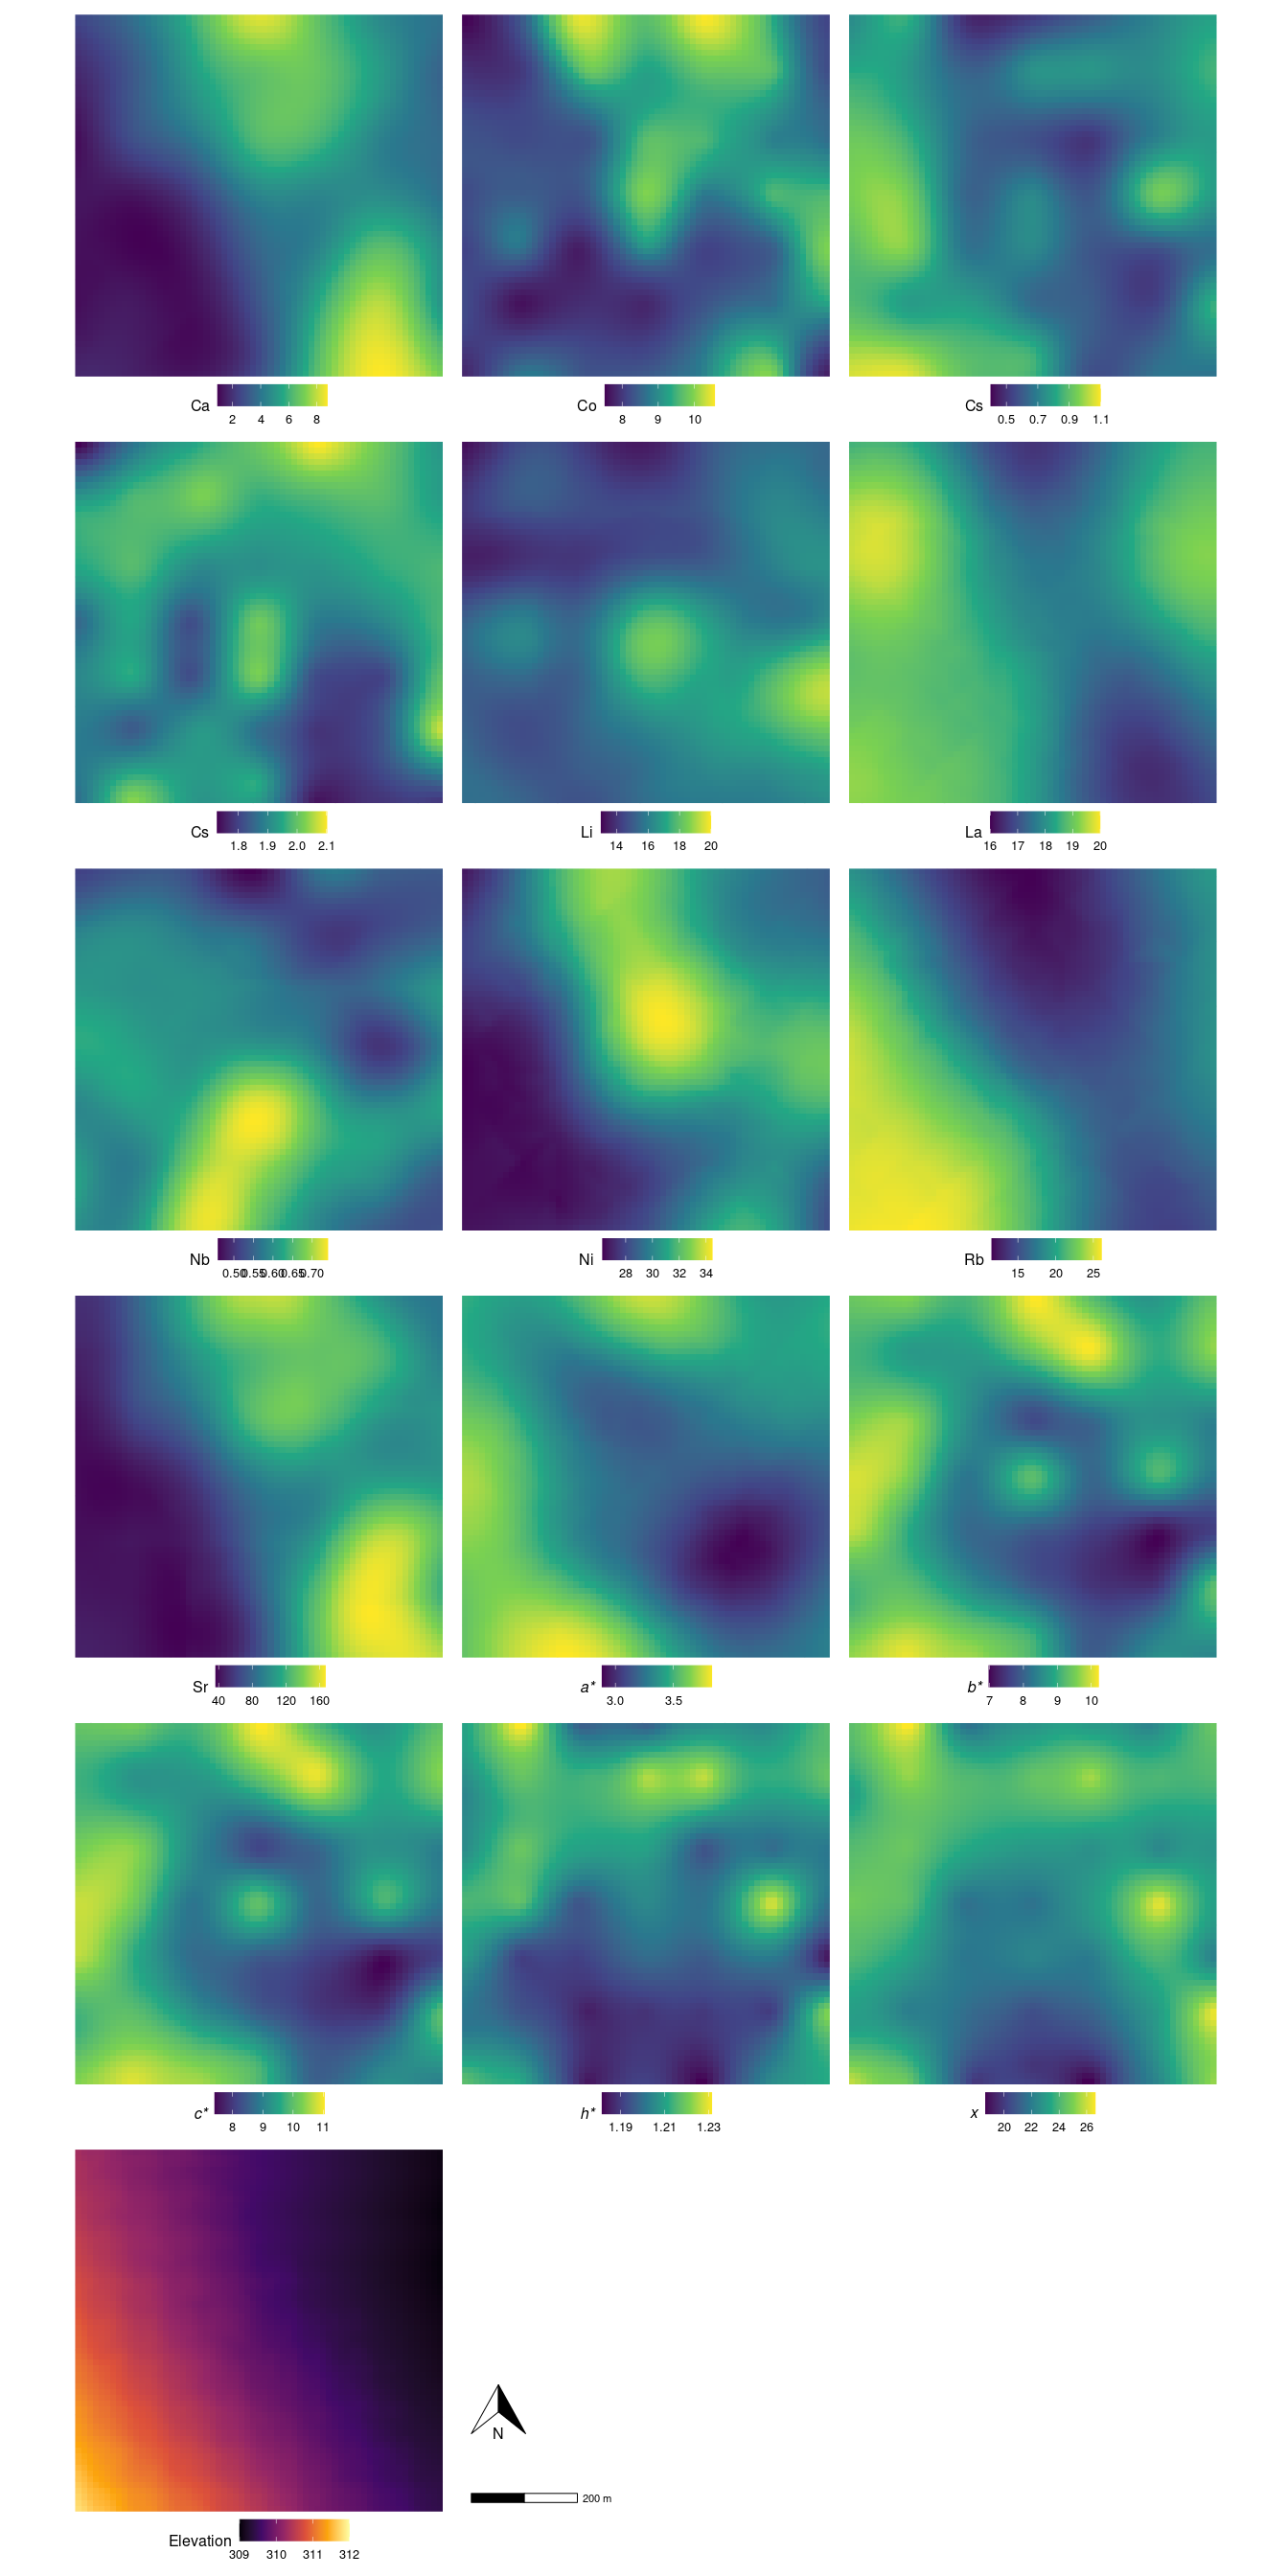
\includegraphics{index_files/figure-latex/notebooks-property_maps-fig-ag_map-output-1.png}

}

\caption{\label{fig-ag_map}Kriged maps of select colour and geochemical
properties and elevtion across the agricultural site.}

\end{figure}%

\textsubscript{Source:
\href{https://alex-koiter.github.io/spatial-variability-soil-manuscript/notebooks/property_maps.qmd.html\#cell-fig-ag_map}{Soil
property mapping}}

\begin{figure}[H]

\centering{

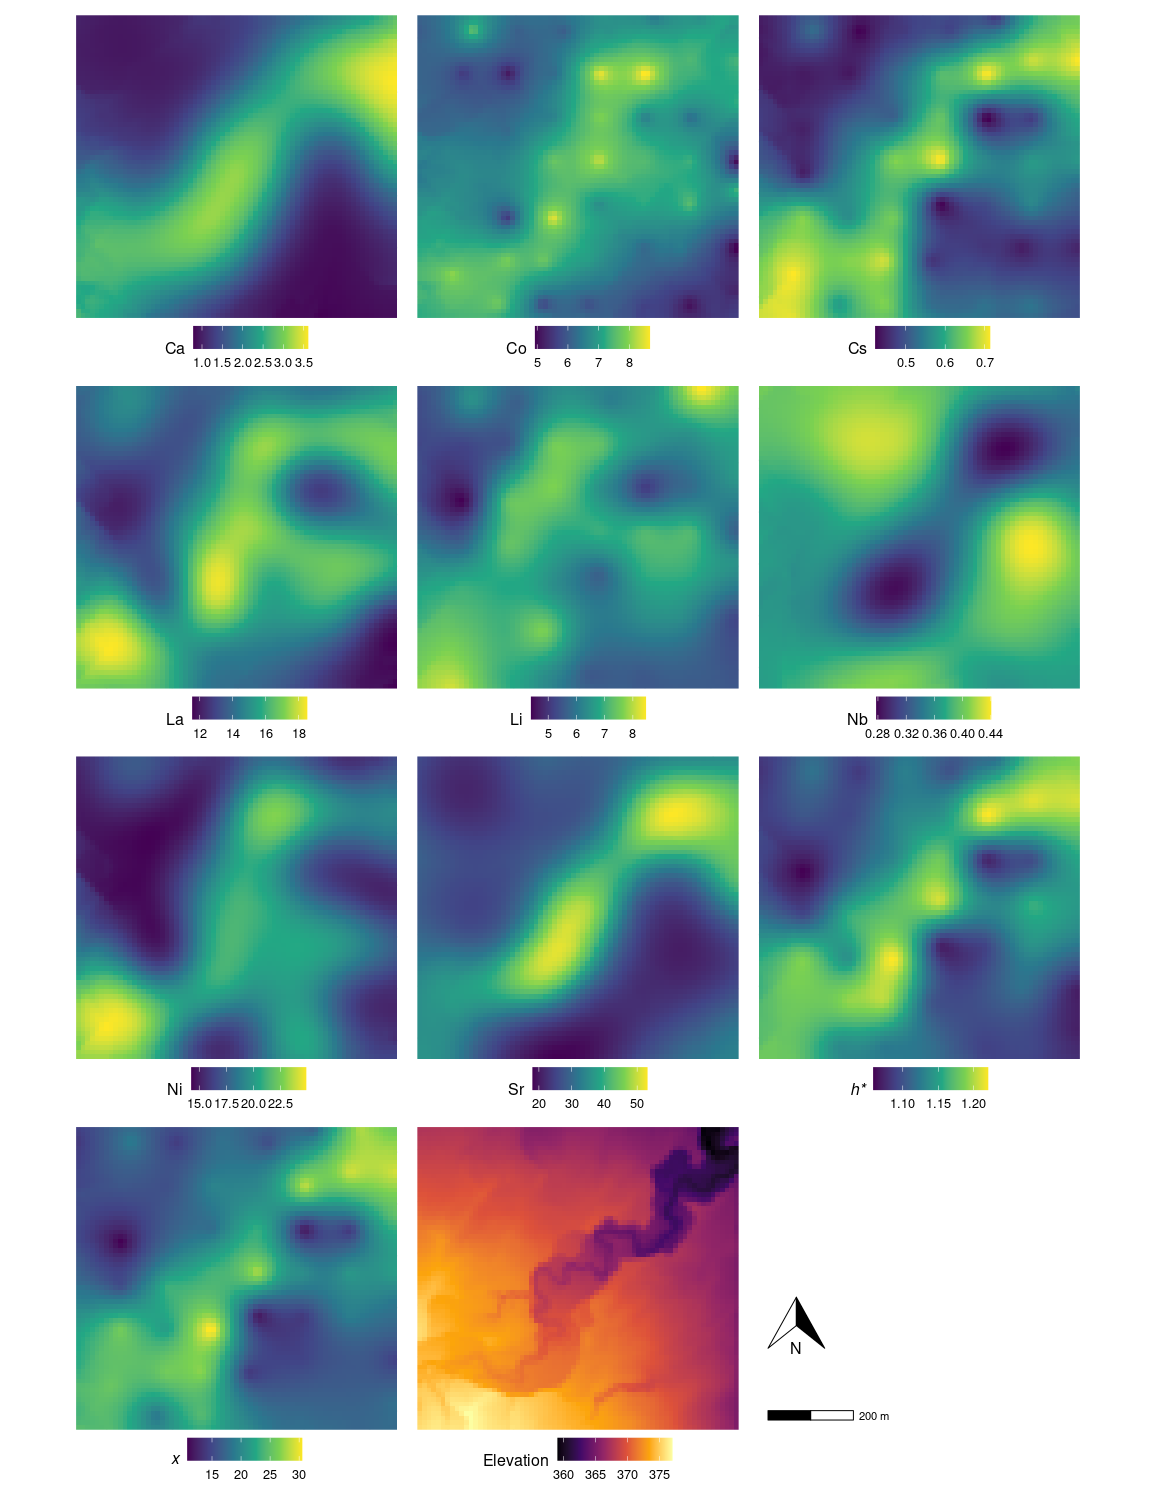
\includegraphics{index_files/figure-latex/notebooks-property_maps-fig-forest_map-output-1.png}

}

\caption{\label{fig-forest_map}Kriged map of select colour and
geochemical properties and elevation across the forested site.}

\end{figure}%

\textsubscript{Source:
\href{https://alex-koiter.github.io/spatial-variability-soil-manuscript/notebooks/property_maps.qmd.html\#cell-fig-forest_map}{Soil
property mapping}}

\begin{figure}[H]

\centering{

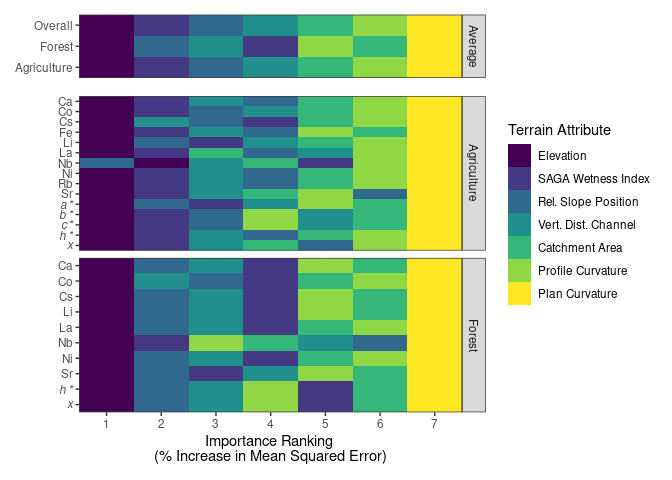
\includegraphics{index_files/figure-latex/notebooks-RF_summary-fig-rf-results-output-1.png}

}

\caption{\label{fig-rf-results}Heat map of the Random Forest regresssion
results showing the ranking of the importance of terrain attributes
(based on \% increase in Mean Squared Error) in explaining the spatial
variabilty of selected colour and geochemical properties within the
agricultural and forested sites. Top panel shows an average ranking for
each site and across both sites.}

\end{figure}%

\textsubscript{Source:
\href{https://alex-koiter.github.io/spatial-variability-soil-manuscript/notebooks/RF_summary.qmd.html\#cell-fig-RF-results}{Random
Forest summary}}

\begin{longtable}[]{@{}
  >{\centering\arraybackslash}p{(\columnwidth - 10\tabcolsep) * \real{0.1667}}
  >{\centering\arraybackslash}p{(\columnwidth - 10\tabcolsep) * \real{0.1667}}
  >{\centering\arraybackslash}p{(\columnwidth - 10\tabcolsep) * \real{0.1667}}
  >{\centering\arraybackslash}p{(\columnwidth - 10\tabcolsep) * \real{0.1667}}
  >{\centering\arraybackslash}p{(\columnwidth - 10\tabcolsep) * \real{0.1667}}
  >{\centering\arraybackslash}p{(\columnwidth - 10\tabcolsep) * \real{0.1667}}@{}}

\caption{\label{tbl-rf-summary}Model summary and performance statistics
for the random forest regression using the training, validation, and
test data sets.}

\tabularnewline

\toprule\noalign{}
\begin{minipage}[b]{\linewidth}\raggedright
Property
\end{minipage} & \begin{minipage}[b]{\linewidth}\raggedright
MSE\\
Training{\textsuperscript{1}}\strut
\end{minipage} & \begin{minipage}[b]{\linewidth}\raggedright
\% Var\\
Training{\textsuperscript{2}}\strut
\end{minipage} & \begin{minipage}[b]{\linewidth}\raggedright
MSE\\
Testing{\textsuperscript{1}}\strut
\end{minipage} & \begin{minipage}[b]{\linewidth}\raggedright
\% Var\\
Validation{\textsuperscript{2}}\strut
\end{minipage} & \begin{minipage}[b]{\linewidth}\raggedright
R{\textsuperscript{2}}\\
Testing\strut
\end{minipage} \\
\midrule\noalign{}
\endhead
\midrule\noalign{}
\multicolumn{6}{@{}>{\centering\arraybackslash}p{(\columnwidth - 10\tabcolsep) * \real{1.0000} + 10\tabcolsep}@{}}{%
{\textsuperscript{1}} Mean square error} \\
\multicolumn{6}{@{}>{\centering\arraybackslash}p{(\columnwidth - 10\tabcolsep) * \real{1.0000} + 10\tabcolsep}@{}}{%
{\textsuperscript{2}} Percent variance explained} \\
\bottomrule\noalign{}
\endlastfoot
\multicolumn{6}{@{}>{\centering\arraybackslash}p{(\columnwidth - 10\tabcolsep) * \real{1.0000} + 10\tabcolsep}@{}}{%
Agriculture} \\
Ca & 0.374 & 91.6 & 0.359 & 91.8 & 0.91 \\
Co & 0.089 & 79.8 & 0.080 & 82.5 & 0.80 \\
Cs & 0.002 & 85.7 & 0.002 & 86.4 & 0.85 \\
Fe & 0.001 & 69.6 & 0.001 & 70.9 & 0.69 \\
Li & 0.538 & 59.3 & 0.533 & 59.8 & 0.64 \\
La & 0.048 & 93.0 & 0.044 & 93.1 & 0.93 \\
Nb & 0.001 & 57.3 & 0.001 & 59.1 & 0.55 \\
Ni & 0.338 & 93.1 & 0.335 & 93.7 & 0.93 \\
Rb & 0.733 & 95.3 & 0.643 & 96.1 & 0.95 \\
Sr & 97.221 & 93.5 & 93.970 & 93.6 & 0.93 \\
a* & 0.007 & 85.0 & 0.006 & 86.9 & 0.85 \\
b* & 0.136 & 72.5 & 0.120 & 75.3 & 0.72 \\
c* & 0.155 & 73.2 & 0.136 & 75.9 & 0.73 \\
h* & 0.000 & 58.3 & 0.000 & 58.6 & 0.56 \\
x & 0.628 & 61.9 & 0.701 & 61.8 & 0.59 \\
\multicolumn{6}{@{}>{\centering\arraybackslash}p{(\columnwidth - 10\tabcolsep) * \real{1.0000} + 10\tabcolsep}@{}}{%
Forest} \\
Ca & 0.231 & 61.1 & 0.231 & 60.7 & 0.63 \\
Co & 0.244 & 39.1 & 0.234 & 42.9 & 0.48 \\
Cs & 0.002 & 64.1 & 0.002 & 67.1 & 0.66 \\
Li & 0.278 & 41.3 & 0.282 & 42.0 & 0.46 \\
La & 1.401 & 43.3 & 1.323 & 47.5 & 0.48 \\
Nb & 0.001 & 55.0 & 0.001 & 55.9 & 0.58 \\
Ni & 2.819 & 55.2 & 2.806 & 56.0 & 0.55 \\
Sr & 29.427 & 59.4 & 29.663 & 59.1 & 0.59 \\
h* & 0.001 & 58.8 & 0.001 & 60.3 & 0.62 \\
x & 5.646 & 62.6 & 5.810 & 63.4 & 0.64 \\

\end{longtable}

\textsubscript{Source:
\href{https://alex-koiter.github.io/spatial-variability-soil-manuscript/notebooks/RF_summary.qmd.html\#cell-tbl-RF-summary}{Random
Forest summary}}

\section*{References}\label{references}
\addcontentsline{toc}{section}{References}

\renewcommand{\bibsection}{}
\bibliography{references.bib}

\section*{Supplemental materials}\label{supplemental-materials}
\addcontentsline{toc}{section}{Supplemental materials}

\phantomsection\label{ssuppfig-geo_summary}
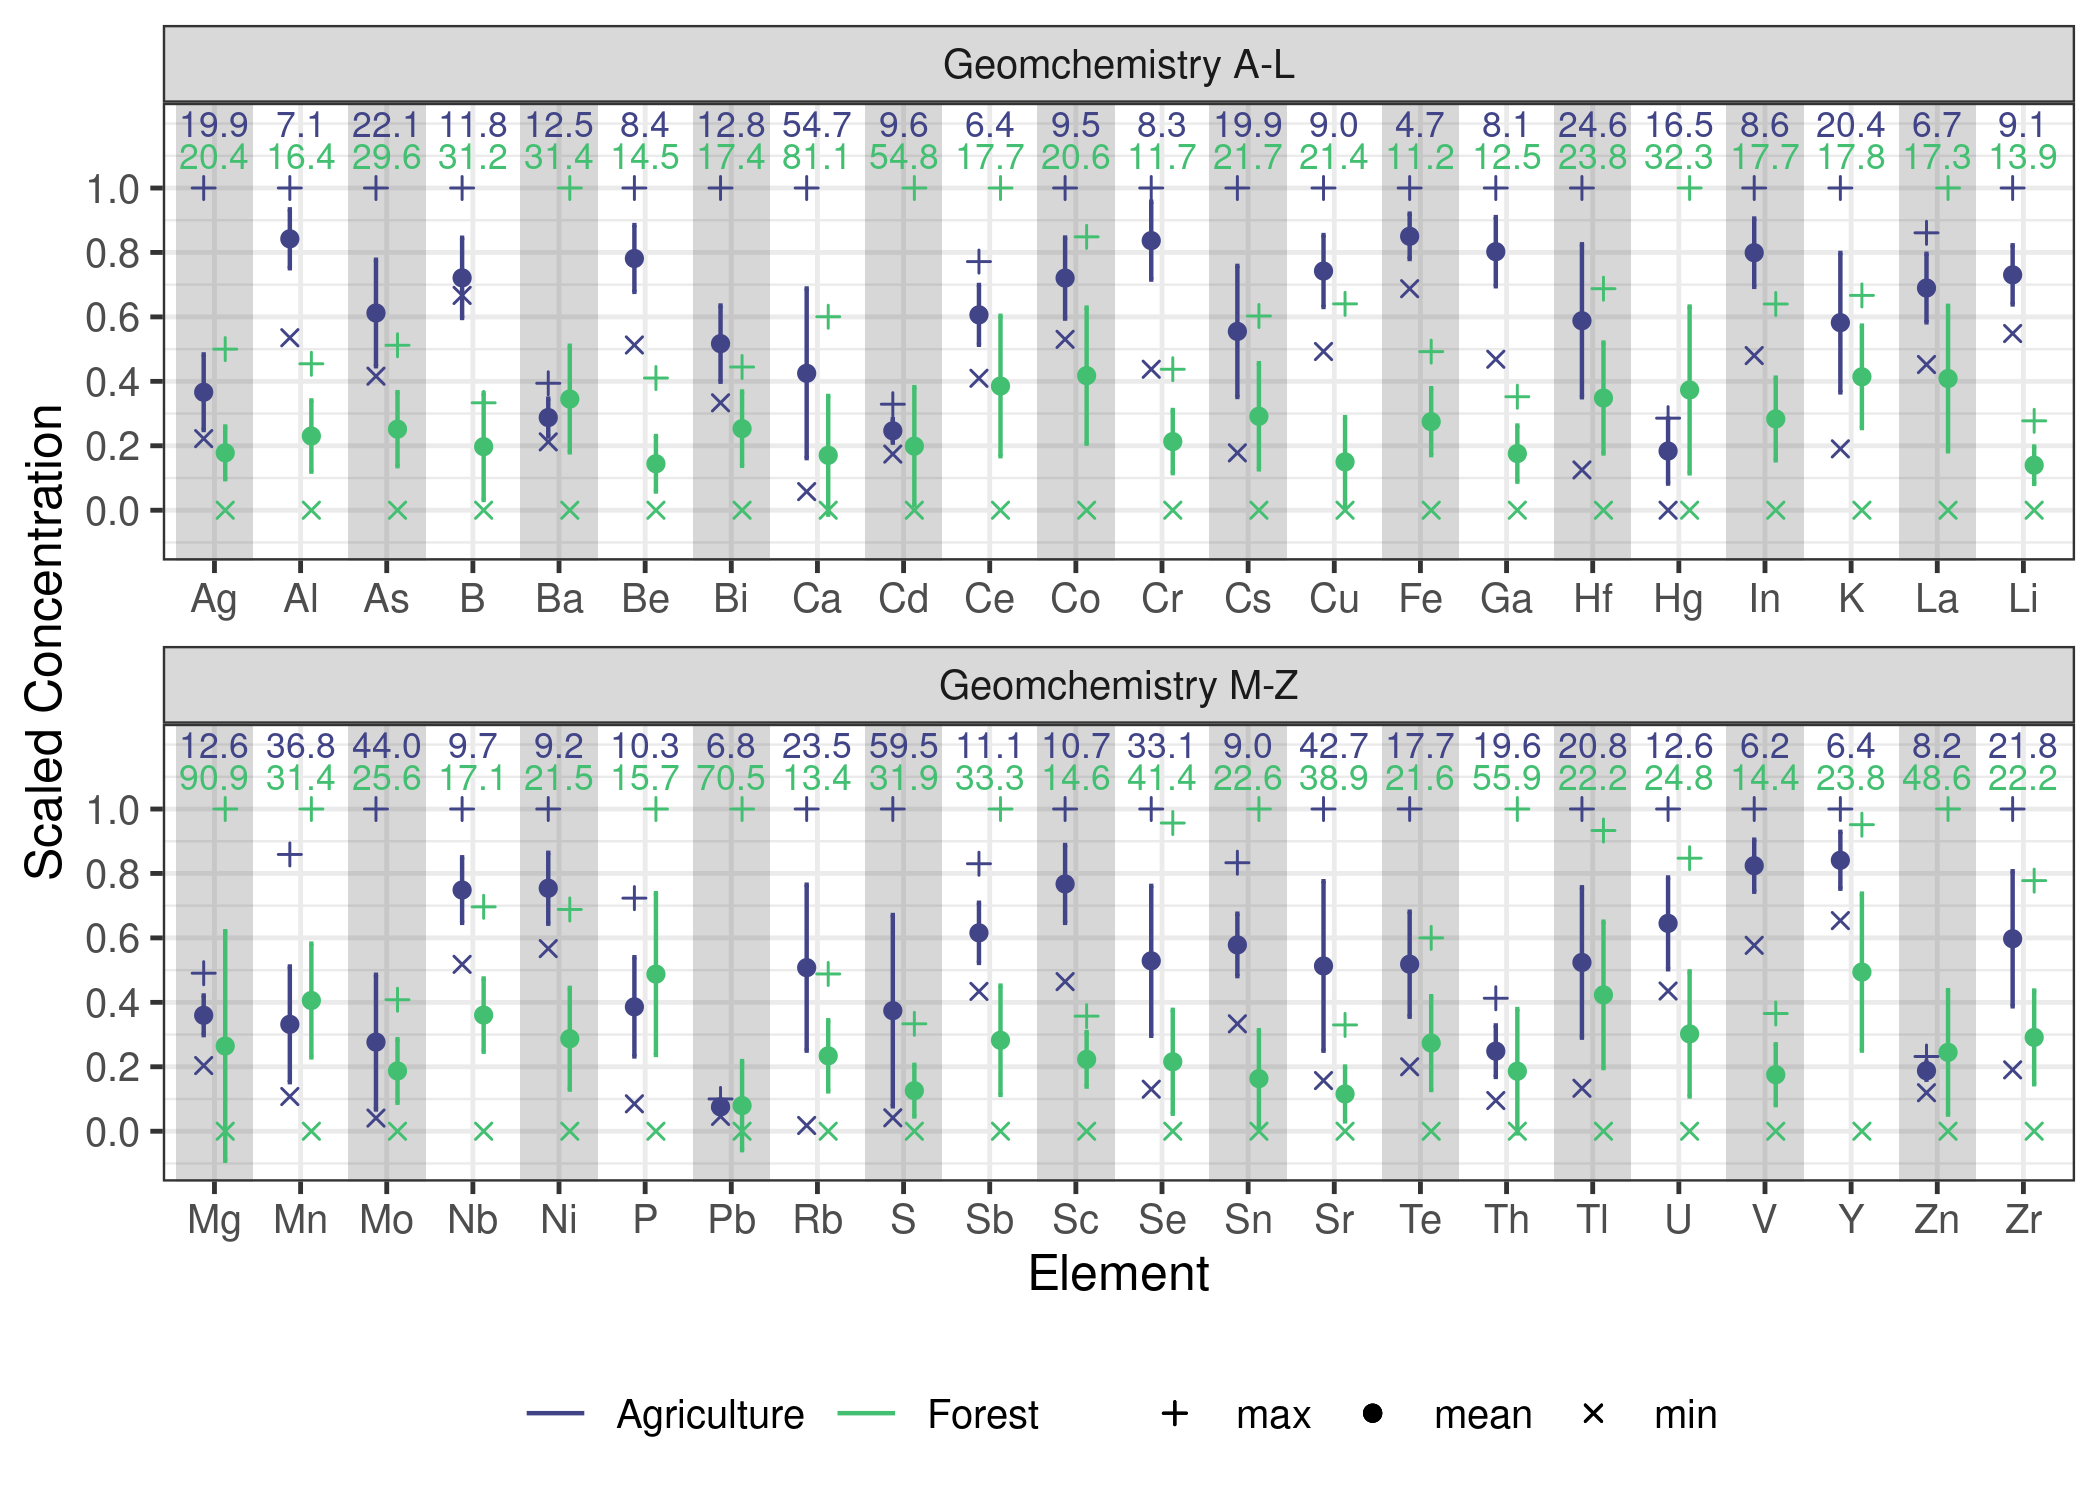
\includegraphics[width=1\textwidth,height=\textheight]{images/geo_summary.png}

Summary statistics of all measured geochemical soil properties at both
sites. Error bars represent 1SD and the numeric values indicate the CV.

\phantomsection\label{ssuppfig-colour_summary}
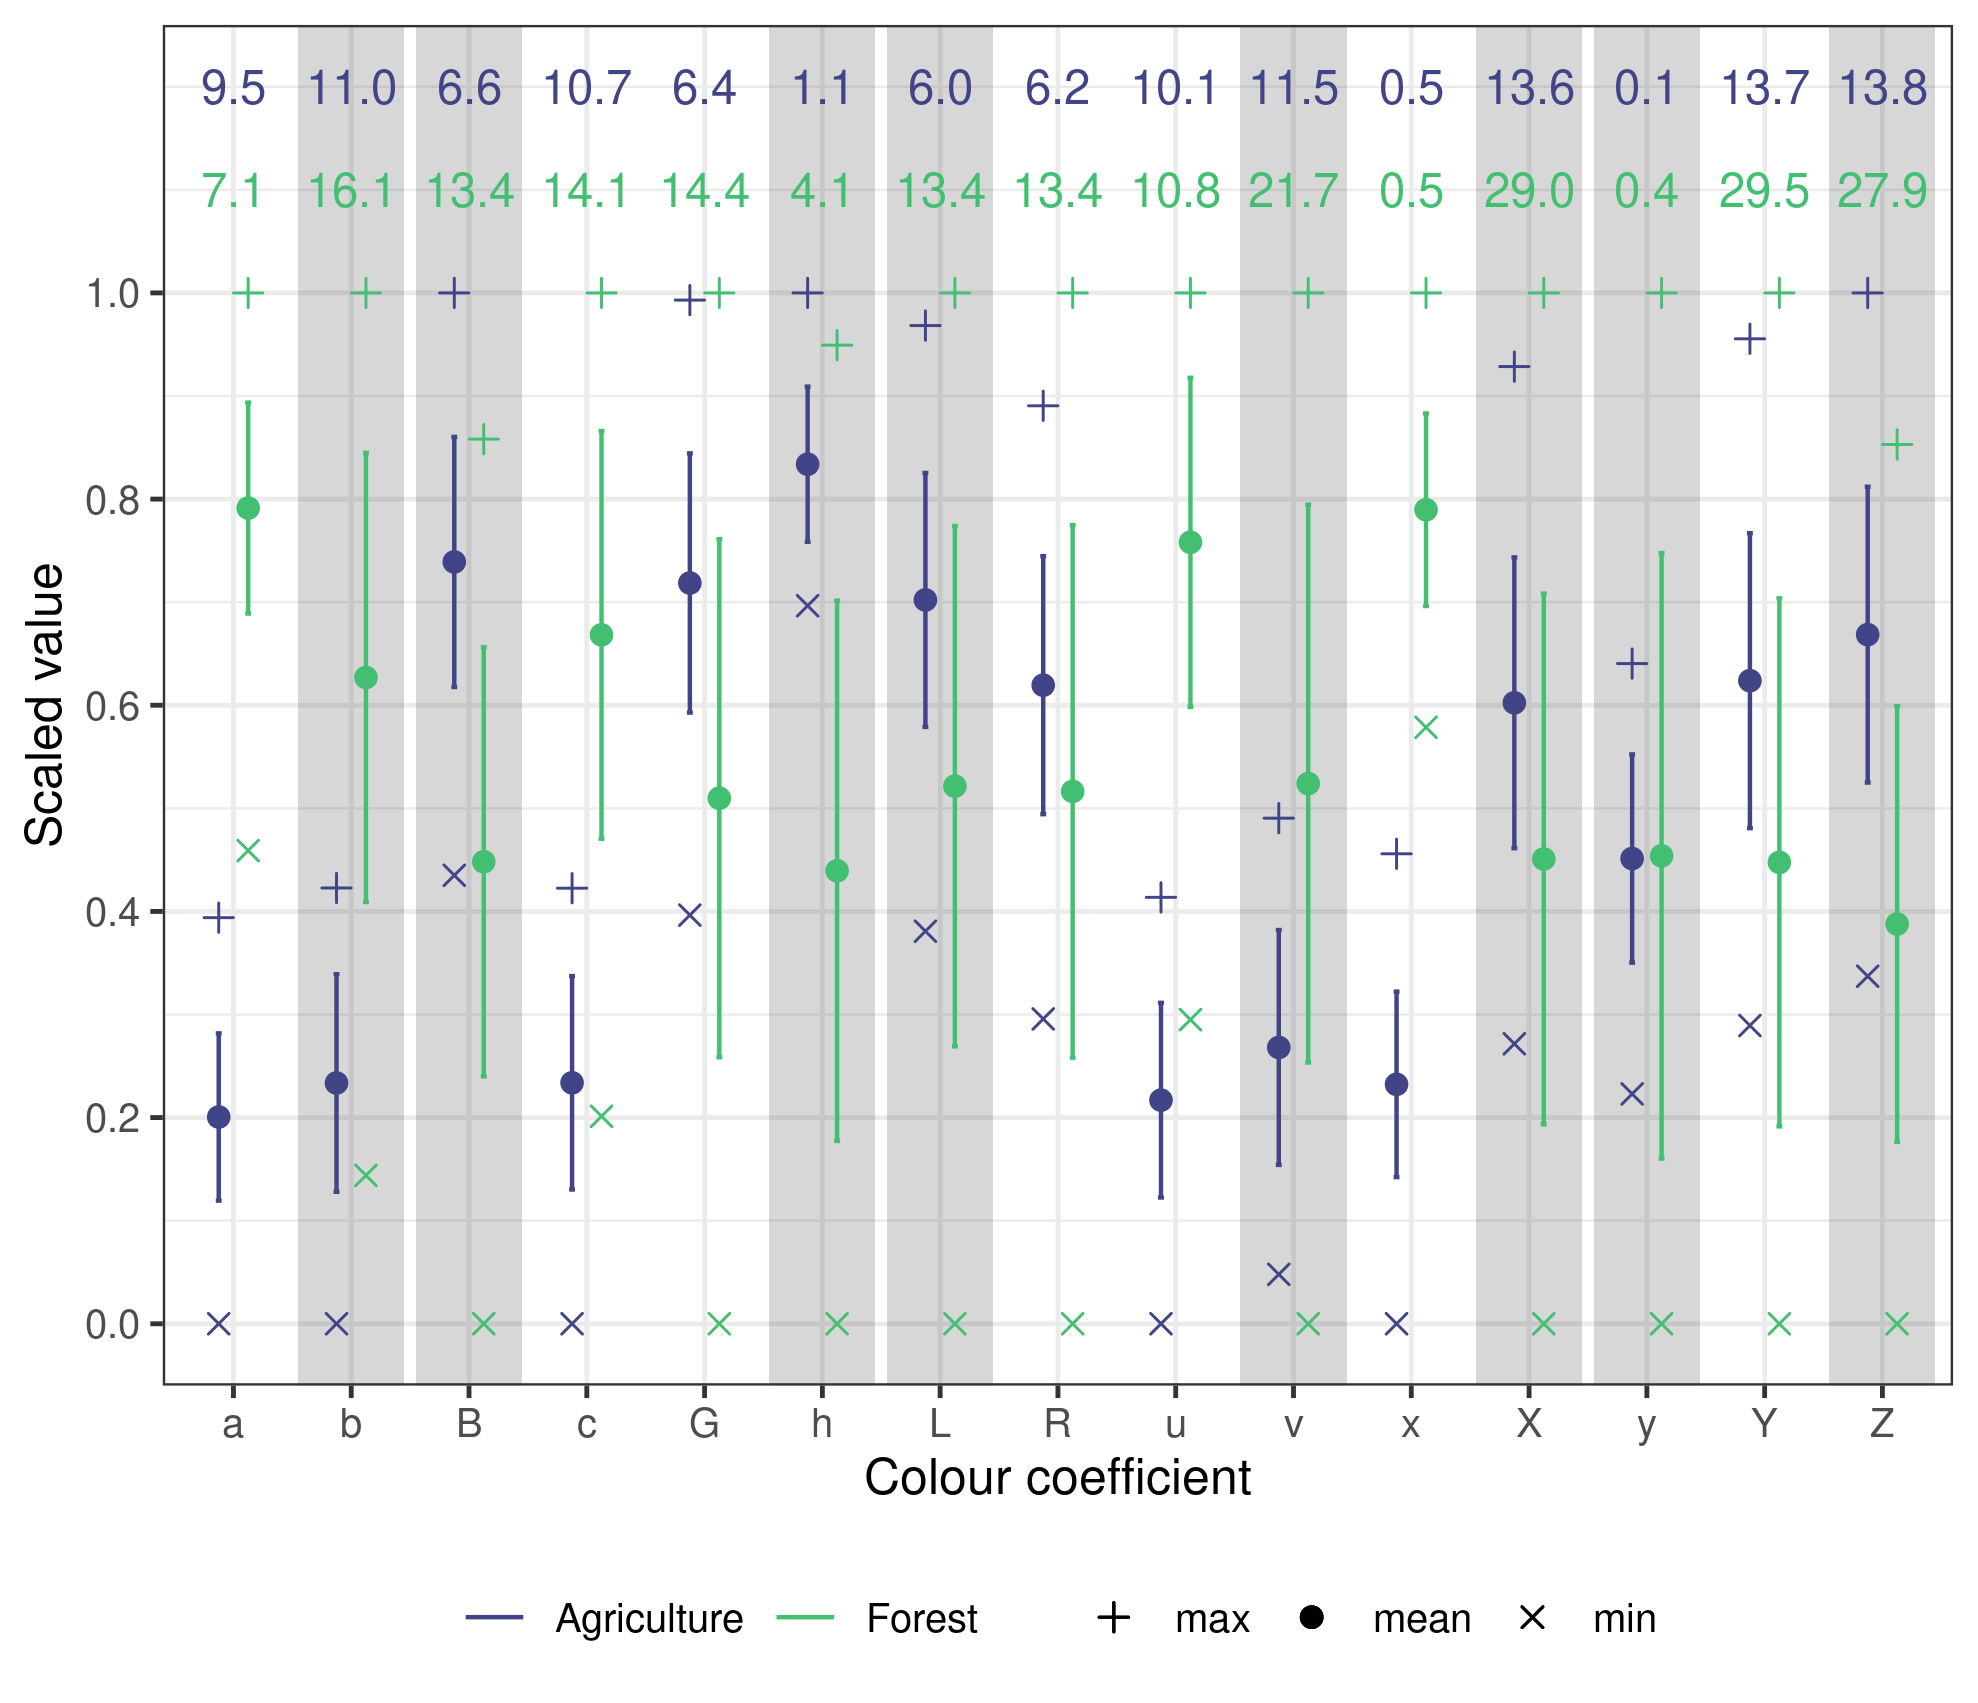
\includegraphics[width=1\textwidth,height=\textheight]{images/colour_summary.png}

Summary statistics of all measured colour soil properties at both sites.
Error bars represent 1SD and the numeric values indicate the CV.

\phantomsection\label{supptab-corr-summary}
\setlength{\LTpost}{0mm}
\begin{longtable*}{llrlrlll}
\toprule
Property & Elevation & SAGA Wetness Index & Rel. Slope Position & Vert. Dist. Channel & Catchment Area & Plan Curvature & Profile Curvature \\ 
\midrule\addlinespace[2.5pt]
\multicolumn{8}{l}{Agriculture} \\ 
\midrule\addlinespace[2.5pt]
Ca & -0.76*** & 0.59*** & -0.26*** & -0.25*** & 0.1*** & NS & NS \\ 
Co & -0.63*** & 0.61*** & -0.23*** & -0.24*** & 0.14*** & NS & NS \\ 
Cs & 0.58*** & -0.45*** & 0.06*** & 0.14*** & -0.11*** & NS & NS \\ 
Fe & -0.14*** & 0.32*** & -0.09*** & -0.09*** & 0.09*** & NS & NS \\ 
Li & -0.4*** & 0.27*** & -0.42*** & -0.2*** & 0.13*** & NS & NS \\ 
La & 0.53*** & -0.3*** & 0.07*** & 0.15*** & NS & NS & NS \\ 
Nb & 0.48*** & -0.52*** & 0.25*** & 0.15*** & -0.08*** & NS & NS \\ 
Ni & -0.75*** & 0.71*** & -0.32*** & -0.32*** & 0.2*** & NS & NS \\ 
Rb & 0.81*** & -0.71*** & 0.24*** & 0.3*** & -0.15*** & NS & NS \\ 
Sr & -0.81*** & 0.64*** & -0.35*** & -0.27*** & 0.12*** & NS & NS \\ 
\emph{a}* & 0.61*** & -0.44*** & 0.35*** & 0.23*** & -0.12*** & NS & NS \\ 
\emph{b}* & 0.39*** & -0.22*** & 0.22*** & 0.1*** & -0.09*** & NS & NS \\ 
\emph{c}* & 0.41*** & -0.24*** & 0.22*** & 0.11*** & -0.09*** & NS & NS \\ 
\emph{h}* & -0.22*** & 0.31*** & -0.15*** & -0.15*** & NS & NS & NS \\ 
\emph{x} & -0.15*** & 0.25*** & -0.23*** & -0.12*** & NS & NS & NS \\ 
\midrule\addlinespace[2.5pt]
\multicolumn{8}{l}{Forest} \\ 
\midrule\addlinespace[2.5pt]
Ca & -0.11*** & -0.47*** & 0.09*** & 0.4*** & 0.24*** & 0.1*** & NS \\ 
Co & -0.04* & -0.34*** & 0.05*** & 0.32*** & 0.15*** & 0.05** & -0.03* \\ 
Cs & 0.09*** & -0.4*** & 0.17*** & 0.34*** & 0.18*** & 0.06*** & -0.03* \\ 
Li & 0.1*** & -0.15*** & 0.05*** & 0.18*** & 0.07*** & NS & NS \\ 
La & NS & -0.23*** & NS & 0.24*** & 0.11*** & 0.05*** & NS \\ 
Nb & 0.12*** & 0.46*** & -0.11*** & -0.34*** & -0.21*** & -0.09*** & 0.05*** \\ 
Ni & 0.19*** & -0.27*** & 0.14*** & 0.2*** & 0.04** & NS & NS \\ 
Sr & -0.34*** & -0.44*** & -0.12*** & 0.36*** & 0.26*** & 0.11*** & -0.05** \\ 
\emph{h}* & -0.08*** & -0.36*** & NS & 0.35*** & 0.22*** & 0.08*** & -0.03* \\ 
\emph{x} & -0.04** & -0.38*** & 0.09*** & 0.35*** & 0.22*** & 0.09*** & -0.03* \\ 
\bottomrule
\end{longtable*}
\begin{minipage}{\linewidth}
*** p < 0.001; ** p < 0.01; * p < 0.05; NS = non-significant at p = 0.05\\
\end{minipage}

\textsubscript{Source:
\href{https://alex-koiter.github.io/spatial-variability-soil-manuscript/index.qmd.html}{Article
Notebook}}

Pearson's correlation coefficients for soil properties and terrain
attributes using interpolated values (10m resolution).





\end{document}
